\chapter{Implementierung}
\label{chap:implementierung}
In diesem Kapitel geht es um die Umsetzung der in \Cref{chap:konzept} erarbeiteten
Konzepts. Da die Arbeit einen CI/CD-Ansatz verfolgt, muss vor der Implementierung
der einzelnen Services die Infrastruktur und die Pipeline umgesetzt werden. 
Wo Tests benötigt werden, werden diese vor der Realisierung der einzelnen
Komponenten verwirklicht. Aufgrund dieser Erkenntnisse, ist das Kapitel der
Implementierung wie folgt gegliedert: In \Cref{sec:infrastruktur} geht es um
die für die Entwicklung, die Testphase sowie die in Produktion laufende Anwendung
benötigten Server. In \Cref{sec:gesamtsysten} geht es um den Aufbau der gesamten
Anwendung. In \Cref{sec:projektaufbau} wird der Aufbau des Projekts behandelt.
In \Cref{sec:pipeline} wird die Implementierung der stetigen Erstellung, Testung und
Auslieferung der Gesamtanwendung beschrieben. In den folgenden Abschnitten wird die
Implementierung der von der Anforderungsanalyse geforderten Features erläutert.
In \Cref{sec:frontendanwendung} wird die Umsetzung der progressiven Webanwendung
mit dem Frontendframework React geschildert. In \Cref{sec:plugins} geht es um die
Implementierung der für die Dashboards benötigten Plugins, die die Daten
in Diagrammen visualisieren. In \Cref{sec:resourcemanagementservice} wird
die testgetriebene Entwicklung der für die Benutzerverwaltung benötigte REST-API
dargestellt. Zuallerletzt wird in \Cref{sec:datadeliveryservice} die Implementierung
des Services geschildert, welcher die Frontendanwendung mit den Daten versorgt.

\section{Infrastruktur}
\label{sec:infrastruktur}
Für die Entwicklung der Gesamtanwendung benötigt die Arbeit einen Linux-Server,
auf dem Gitlab CE, Gitlab Runner und eine Docker Registry
installiert sind. Des Weiteren benötigt es einen Server für die Testphase und mehrere für die
Produktion. Die einzelnen Services werden mit Docker Swarm\footnote{https://docs.docker.com/engine/swarm/},
einem Orchestrierungssystem für Docker-Container, auf dem Produktivsystem ausgeführt. Je nach Skalierung
werden die Instanzen der Services unter den in Produktion laufenden Servern aufgeteilt.
In Zukunft soll die Integration von neuen Servern mithilfe des Open Source IAC-Werkzeugs\footnote{IAC steht für Infrastructure as Code}
Terraform über eine Cloudanbieter-API automatisiert werden.
Die Arbeit beschränkt sich auf vier Linux-Server. Einen für die Versionsverwaltung
und die CI/CD-Prozesse, einen für die Testphase und zwei für das Ausführen der Anwendung in Produktion.
Die vier Server werden von Hetzner, einem Cloudanbieter, bereitgestellt und haben Ubuntu 18.04
vorinstalliert. Der Server für die CI/CD-Prozesse und die Versionsverwaltung besitzt 4 VCPUs, 
16GB RAM und  haben 4 VCPUs, 16GB RAM und 160GB SSD-Speicher.\footnote{Im Regelfall handelt es sich bei
den VCPUs um Intel Skylake Xeon CPUs mit 2.1 GHz.\cite{CPUusedInHetznerCLoud}}
Der Server der Testphase besitzt 2 VCPU, 8GB RAM und 80GB SSD-Speicher. Die für die Produktion
ausgelegten Server besitzten 8 VCPUs, 32GB RAM und 240GB SSD-Speicher.
Die Produktionsserver (Nodes) sind in einen Manager- und einen Worker-Node aufgeteilt. Von dem Manager-Node
aus können Instanzen hinzugefügt und auch wieder entfernt werden. Um die Daten zu persistieren,
ist ein 10GB SSD Volumen an den Manager-Node angebunden. In der Docker-Compose-Datei werden
Regeln definiert, die festlegen, dass die Datenbanken immer auf dem Manager-Server angelegt werden.
Die für die Speicherung der Daten relevanten Ordner der Datenbanken werden auf dem Volumen abgebildet.
Dadurch wird sichergestellt, dass die Daten auf nach dem Herunterfahren des Docker-Clusters noch bestehen.
In Abbildung \ref{figure:dockerswarmcluster} ist das Docker Swarm Cluster der Arbeit zu sehen. Die Schlösser
repräsentieren die Regeln, nach denen sich bestimmte Instanzen auf bestimmten Nodes befinden müssen.
Alle weiteren Instanzen werden nach Auslastung auf die Nodes verteilt. Die Content Delivery (Nginx)
und der Resource Management Service (API) sind auf zwei Instanzen skaliert. Vier Instanzen repräsentieren
den Data Delivery Service (Delivery).

\begin{figure}
    \begin{center}
    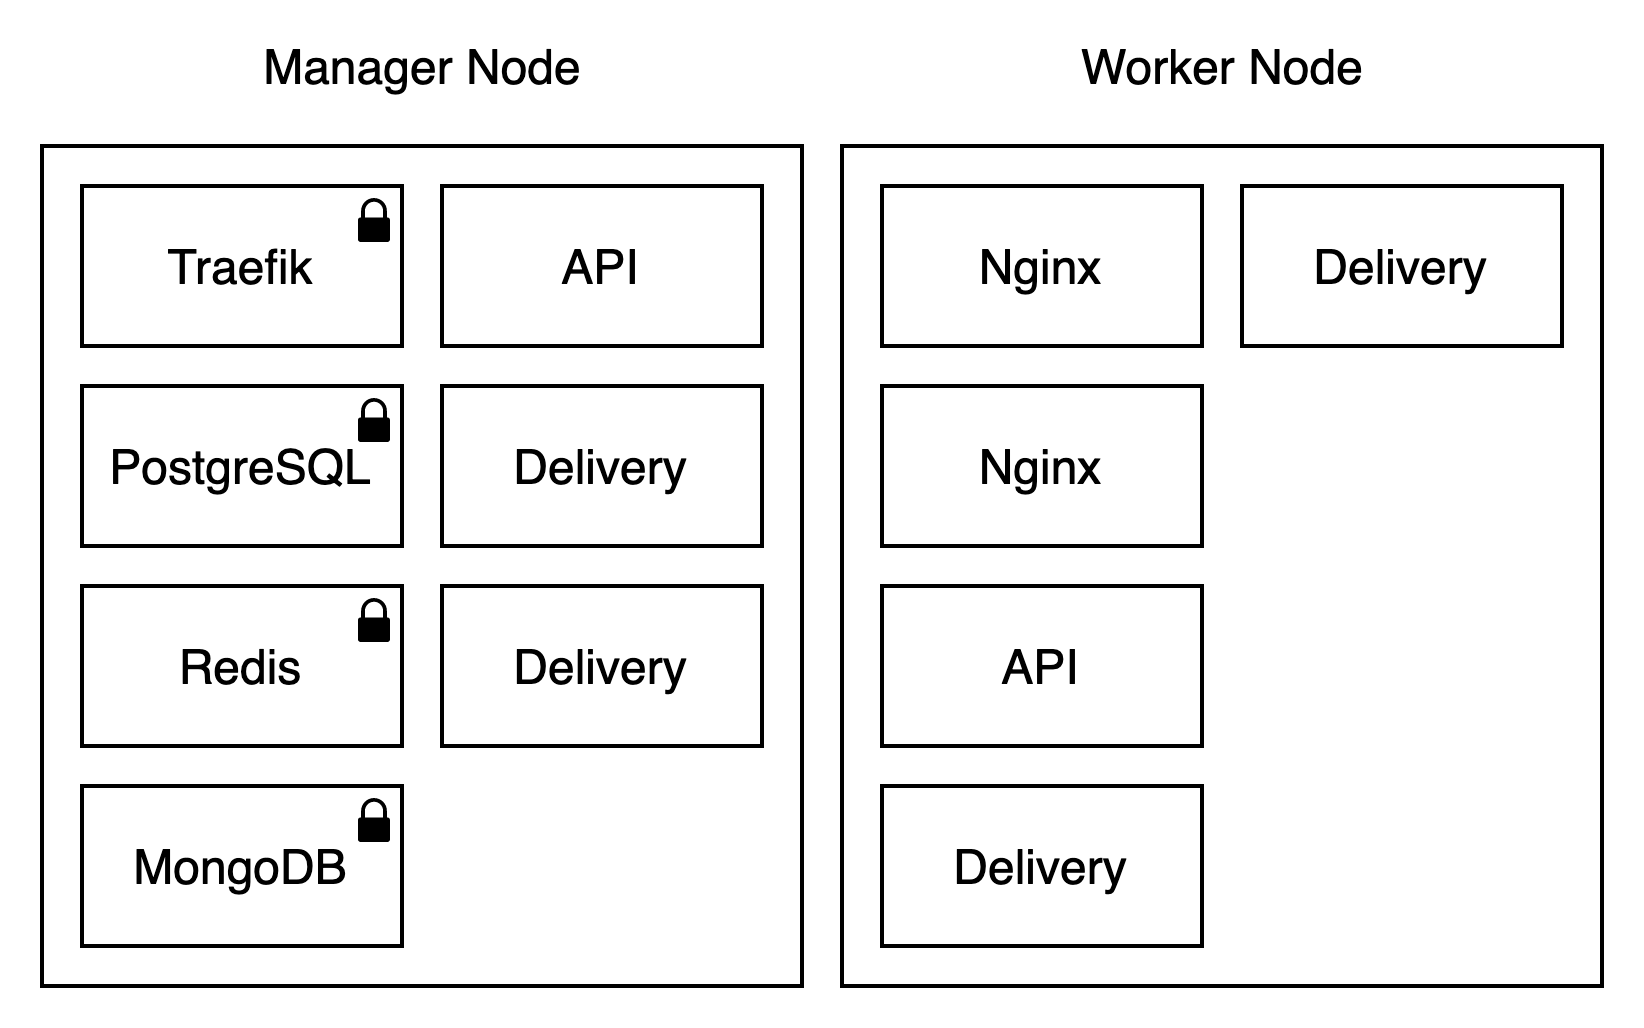
\includegraphics[scale=0.2]{img/abbildungen/Cluster}
    \end{center}
    \caption{Docker Swarm Cluster}
    \label{figure:dockerswarmcluster}
\end{figure}


Um die Server über das Internet zu erreichen, benötigt es Domains
und Subdomains, die mithilfe von DNS-Records auf die vom Server bereitgestellten
IPv4- und IPv6-Adressen verweisen.\footnote{Man kann die Server natürlich auch direkt über
die IP-Adresse ansprechen.} Die Domain \code{blicc.org} dient als
Hauptdomain und wird in der Produktion verwendet. Der Name Blicc
wurde zur Repräsentation des Produktes gewählt. Bei einer Verwendung der Anwendung
als White-Label-Produkt wird der Name durch den der zu repräsentierenden Firma ersetzt.
Der Name Blicc ist eine veränderte Form des deutschen Wortes "Blick". Der Name wurde
daher verändert, da die Verfügbarkeit von "Blick" in den meisten Domainvariationen
nicht mehr erhältlich war oder aber überteuert angeboten wurde. Die Domain für den
Server der Testphase ist \code{testing-stage.org}. Die beiden Domains besitzten die
Subdomains \code{api} und \code{delivery}. Die Subdomain \code{api} verweist auf
den Resource Management Service; die Subdomain \code{delivery} auf die Data Delivery Service.
Außerdem gibt es die \code{monitor} Subdomain, welche auf die Kontrollübersicht von Traefik
verweist. Traefik dient als Reverse-Proxy und bietet zusätzlich rudimentäre
Überwachungsfunktionalitäten in einem webbasierten Dashboard an.
Dazu mehr in \Cref{subsec:reverseproxyundloadbalancer}.

Die Docker Registry ist unter der Domain \code{registry.thiloilg.com}, Gitlab CE
unter \code{gitlab.thiloilg.com} erreichbar. Die Repositories werden alle zusätzlich
auf Github gespiegelt. Github dient als drittes Backup, falls die Repositories auf dem
eigenen Gitlab Server und dem lokale Rechner verloren gehen. Mit dem Git-Befehl in
Quellcode \ref{lst:gitalias} kann ein Alias gesetzt werden, um zu allen Remote Repositories
gleichzeitig zu pushen. Der senkrechte Strich im Linux Terminal, bekannt als "Pipe",
trennt zwei Befehle in der Kommandozeile. Das Ergebnis des ersten Befehls wird
an den zweiten Befehl weitergereicht.

\begin{listing}
    \inputminted{sh}{snippets/sh/pushall.sh}
    \caption{Konfiguration eines eigenen Git Alias}
    \label{lst:gitalias}
\end{listing}

Für das Aufsetzen der Server benötigt man drei Schritte.
Als erstes verbindet man sich über SSH zu dem Server und richtet eine Firewall ein.
Hierfür verwendet die Arbeit UFW, eine in Ubuntu vorinstallierte
Firewall.\footnote{UFW steht für Uncomplicated Firewall} Dabei öffnet man alle Ports,
die von den Anwendungen des Server benötigt werden. Aufgrunddessen, dass bei dem Gitlab CE Server
Port 22 bereits für die SSH verbindung benötigt wird, musste der Gitlab Shell SSH
Port auf 2222 verlegt werden. In der Tabelle \ref{tab:geoeffneteportsderproduktionsserver}
sieht man die geöffneten Ports der Produktionsserver.

\begin{table}[h]
    \begin{center}
\begin{tabular}{rll}
PORT & Protokoll & Verwendungszweck\\
\hline
22 & TCP & SSH\\
80 & TCP & HTTP/WS\\
443 & TCP & HTTPS/WSS\\
2377 & TCP & Kommunikation zwischen Nodes\\
4789 & UDP & Ingress Netzwerk\\
7946 & TCP/UDP & Kommunikation zwischen Instanzen\\
\end{tabular}
\end{center}
\caption{Geöffnete Ports der Produktionsserver}
\label{tab:geoeffneteportsderproduktionsserver}
\end{table}

Als zweiten Schritt werden Docker CE und Docker-Compose auf dem Server installiert.
Als dritten Schnitt wird der Befehl \code{docker swarm init} auf dem Manager-Server
ausgeführt. Die Worker-Server werden daraufhin mit dem Manager-Server verbunden.
Die restlichen Schritte sind alle von der Pipeline aus automatisiert. Die Pipeline
kopiert mithilfe von SCP die \code{docker-compose.yml} Datei auf den Manager-Server,
logt sich in die Docker Registry ein, zieht die neuen Images und startet das Cluster.
Mehr dazu in \Cref{sec:pipeline}.

\section{Gesamtsystem}
\label{sec:gesamtsysten}
In diesem Abschnitt wird aus dem Konzept ein komplettes System
entwickelt. Der Abschnitt fokussiert sich auf die Merkmale der Komponenten,
die für das Gesamtsystem relevant sind. In \Cref{subsec:systemuebersicht} verschafft
sich die Arbeit einen groben Überblick über das System. Anhand einer Grafik wird das Zusammenspiel
der einzelnen Komponenten erläutert. In  \Cref{subsec:reverseproxyundloadbalancer}
wird der Reverse Proxy und der Load Balancer behandelt. In \Cref{subsec:inhaltsauslieferung} wird
die Inhaltsauslieferung vorgestellt. Dabei stellt sich die Frage,
wie die Ressourcen möglichst performant an die Clients transportiert
werden können. In \Cref{subsec:wahlderdatenbankarten} geht es um die Wahl
der Datenbankart der einzelnen Services. Abschließend setzt sich die Arbeit
in \Cref{subsec:ueberwachungundwartung} mit der Überwachung und Wartung
des Systems auseinander.

\subsection{Systemübersicht}
\label{subsec:systemuebersicht}
Die Abbildung \ref{figure:uebersichtueberdassystem} verschafft einen guten Überblick
über das Zusammenspiel der einzelnen Komponenten. Im oberen Bereich sieht man die
Frontendanwendung sowie eine Repräsentation einer externen API. Die Frontendanwendung
besteht aus dem Frontend sowie dem integrierten Plugin-System. Je nach Kommunikationsart
unterhält sich das Frontend über HTTPS oder WSS mit dem Backend. Die HTTPS-Kommunikation
wird durch einen Service Worker interferiert, um das Frontend-Caching und die
Offline-Funktionalität zu ermöglichen. Das WebSocket-Protokoll verbindet das Frontend
über direktem Web mit dem Backend. Dies kann allerdings von Browser zu Browser variieren.
Mache Versionen der Browser enthüllen die WebSocket-Kommunikation im SW, andere
nicht.\footnote{Siehe Diskussion auf Github, W3C Service Worker \cite{GithubIssueWebSocketExpose}}
Die Kommunikation zwischen externen APIs und dem Backend kann über HTTP als auch
HTTPS erfolgen. Zukünftige Kommunikationen über WebSockets oder QUIC\footnote{QUIC (Quick UDP Internet Connections) ist ein von Google entwickeltes, auf UDP basierendes Transportprotokoll.\cite{IETFQUICWhatsHappening} Die IETF arbeitet an einer Standardisierung des Internetprotokolls.\cite{DatatrakcerIETFQuic}}
sind denkbar.

\begin{figure}
    \begin{center}
    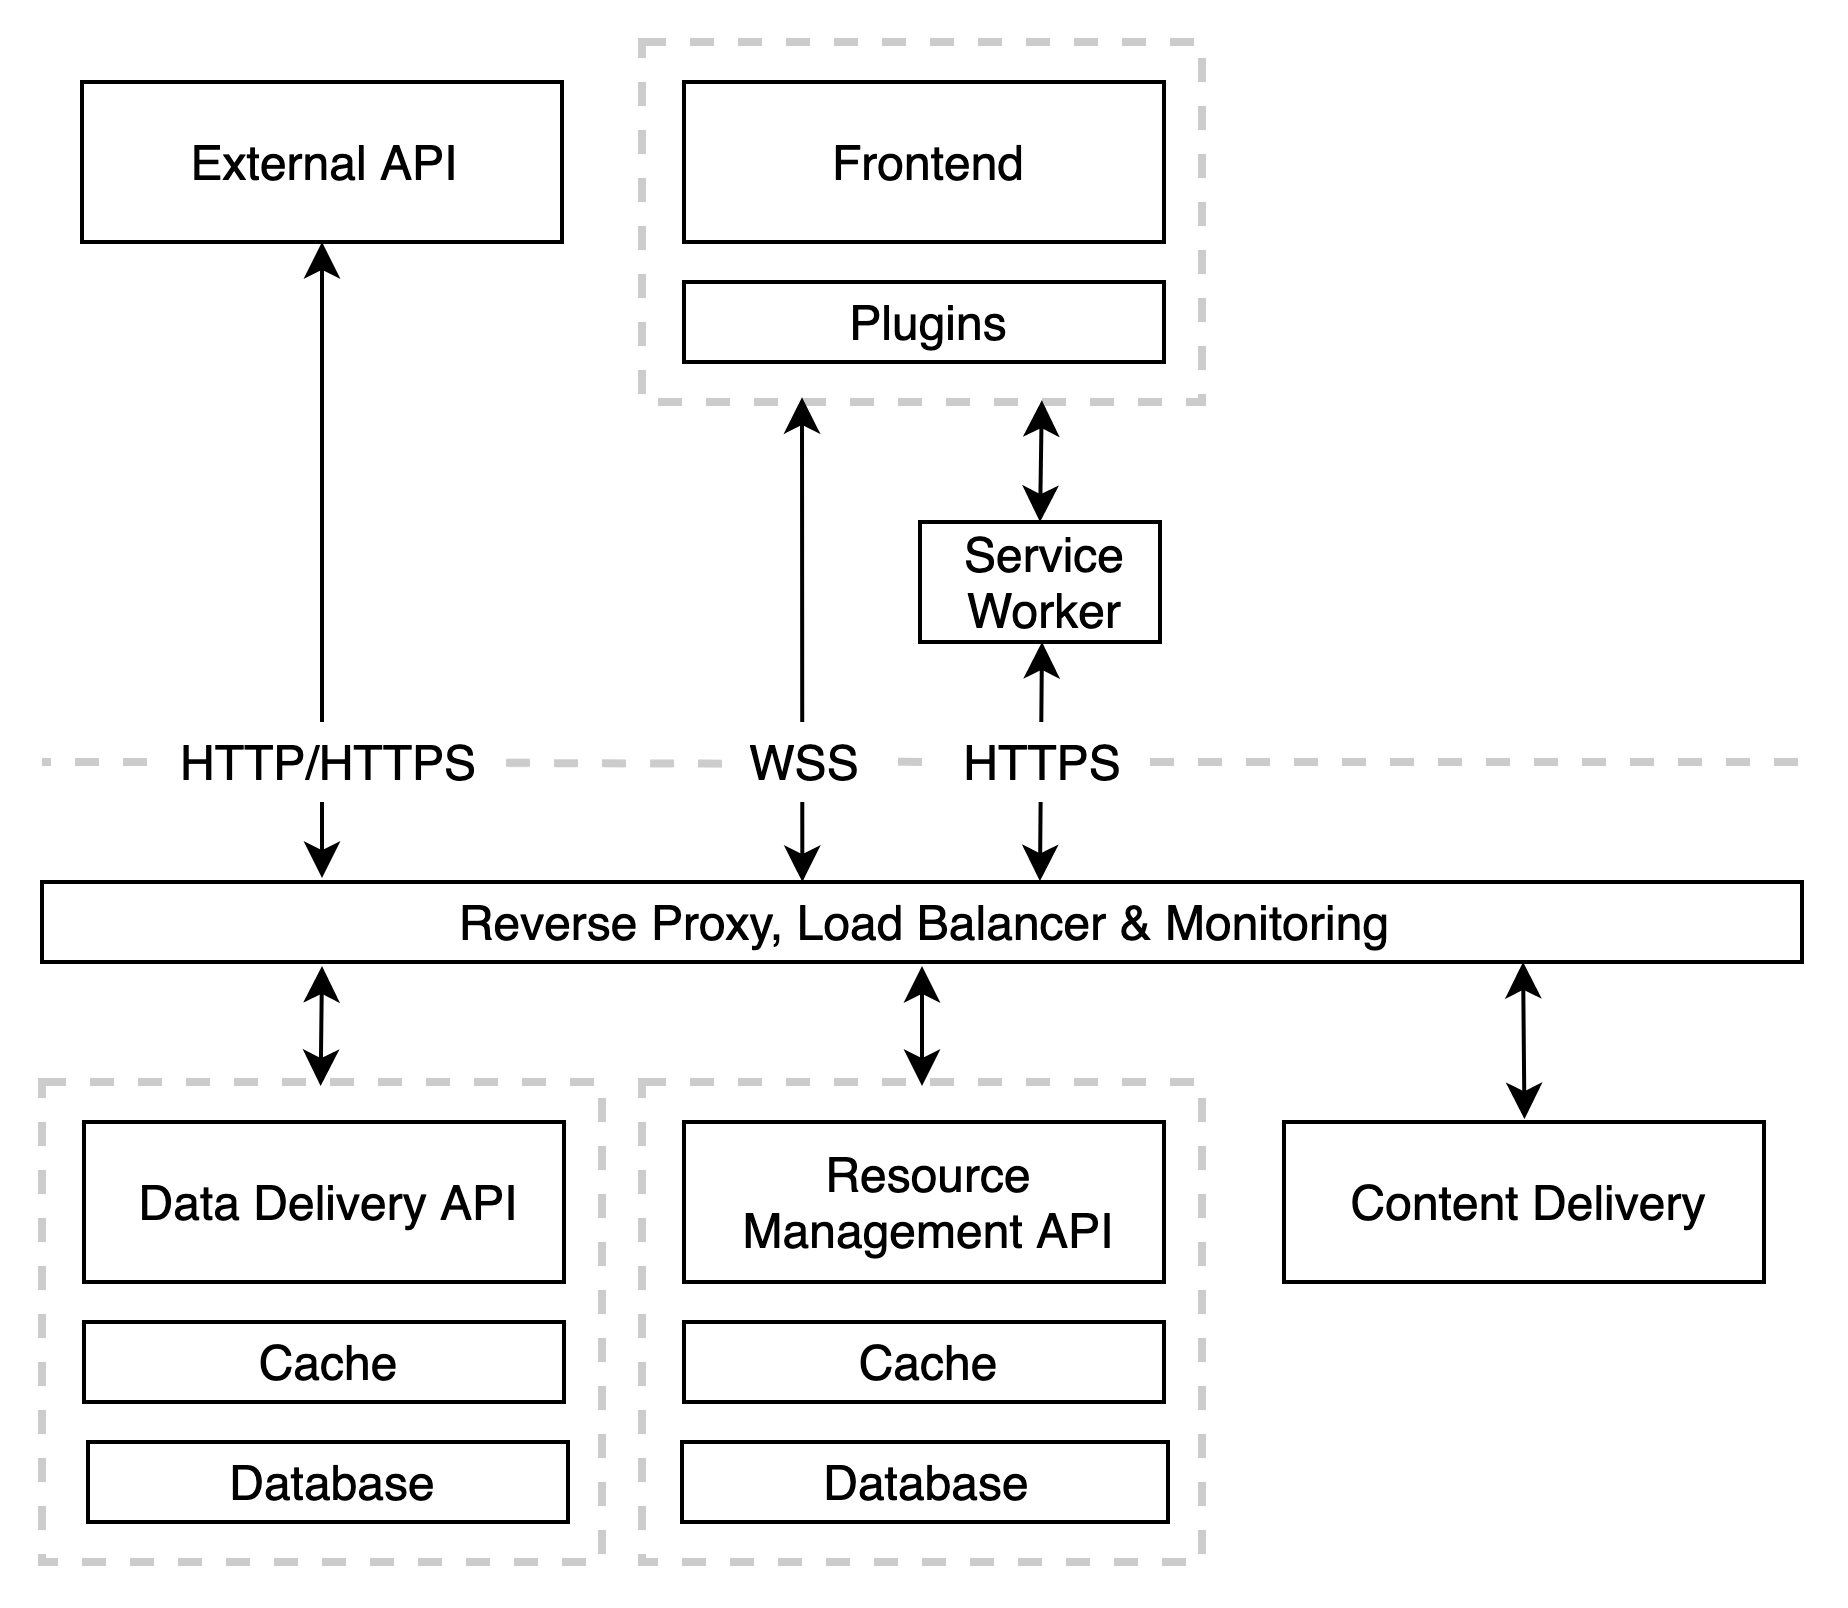
\includegraphics[scale=0.2]{img/abbildungen/MicroserviceInfrastruktur}
    \end{center}
    \caption{Übersicht über das System}
    \label{figure:uebersichtueberdassystem}
\end{figure}

Das Backend und dessen Microservice-Infrastruktur wird durch einen Reverse Proxy vom Internet versteckt.
In dieser Zwischenschicht befinden sich unter anderem ein Load Balancer sowie ein Monitoring System.
Das Backend ist in drei Services unterteilt; den Data Delivery Service, den Resource Management Service
und den Content Delivery Service. Der Data Delivery Service sowie der Resource Management Service sind jeweils
in drei Container unterteilt. Der wichtigste Container führt die Servicelogik aus. In der zweiten
Schicht befindet sich eine In-Memory-Datenbank, die für das Caching verantwortlich ist. Zuallerletzt
kommt eine Datenbank, um den Fortbestand der Daten zu sichern. Die Caching-Strategie sowie die Art der
Datenbank variiert je nach Anforderung an den Service. Für die Langzeitspeicherung der Daten wird je nach Service
eine dokumentenorientiertes als auch ein relationales Datenbanksystem verwendet. Der Content Delivery Service
ist für die Auslieferung der statischen Dateien des Frontends verantwortlich.

\subsection{Reverse Proxy und Load Balancer}
\label{subsec:reverseproxyundloadbalancer}
Anders, als bei einem Proxy, der den Client von dem Server versteckt, versteckt ein Reverse Proxy
eine Serverinfrastruktur vor dem Client. Durch die Anonymisierung der Serverinfrastruktur
sind Angriffe gegen spezifische Servertechnologien erschwert, da deren Schnittstelle
nicht direkt mit der Außenwelt kommuniziert. Als Reverse Proxy verwendet die Arbeit
die in Golang geschriebene Open Source Software Traefik.\footnote{https://docs.traefik.io/}
Neben der Funktionalität als Reverse Proxy bietet Traefik eine
SSL/TLS-Verschlüsselung über den Service Let's Encrypt an.\footnote{https://letsencrypt.org/}
Laut einer Checklist von Google ist eine Verbindung über HTTPS
Vorraussetzung für die Auslieferung einer PWA.\cite{GooglePWAChecklist}
Ohne SSL/TLS-Verschlüsselung werden Funktionalitäten wie das hinzufügen der App zum Homescreen
von den Browsern nicht bereitgestellt. Verschlüsselungsschichten wie TLS und der Vorgänger
SSL liegen zwischen der TCP-Schicht und HTTP/WS. Neben dem Public-Key-Verschlüsselungsverfahren
muss für eine TLS-Verschlüsselung auch die Authentizität des Servers, mit dem kommuniziert wird,
bestätigt sein. Hierfür wird ein EV-TLS-Zertifikate\footnote{EV steht für Extended Validation} benötigt.
Mithilfe von Let's Encrypt, einer gemeinnützigen Zertifizierungsstelle, werden EV-TLS-Zertifikate
kostenlos über eine API zur Verfügung gestellt. Die Arbeit hat sich für Traefik entschieden,
da der Reverse Proxy einen automatisierten Vorgang bereitstellt, indem die EV-TLS-Zertifikate
kurz vor dem Ablaufdatum über den von Let's Encrypt bereitgestellten Service aktualisiert werden.

Die Aufgabe des Load Balancers übernimmt das Orchestrierungssystem Docker Swarm. Swarm verwendet
als Lastverteilungsverfahren Round-Robin, eine rotierende Verteilung der eingehenden Anfragen auf
die unterschiedlichen Instanzen eines Services.\cite{CloudflareRoundRobinDNS}
Da die Aufrechterhaltung der WebSocket-Verbindungen des Data Delivery Services gegenüber
den Clients allerdings nicht linear verläuft,\footnote{Manche Benutzer beenden die Anwendung sofort, andere lassen Sie über Tage laufen.}
empfiehlt es sich für die Zukunft, die Implementierung eines Lastverteilungsverfahrens
basierend auf Health-Checks zu verwenden. Die Health-Checks könnten so die aktuelle
Auslastung der Instanzen bereitstellen, anhand derer dann die Last gleichmäßig verteilt wird.

\subsection{Inhaltsauslieferung}
\label{subsec:inhaltsauslieferung}
Die Inhaltsauslieferung ist dafür zuständig, statische Inhalte der Frontendanwendung
an den Client auszuliefern. Die statischen Inhalte sind unter anderem
HTML-, CSS- und JS-Dateien, JSON-Dateien wie das Web App Manifest sowie Bilddateien.
Die Arbeit verwendet als zur Inhaltsauslieferung den Webserver Nginx. Für die Kompression der statischen
Inhalte wird Brotli verwendet. Brotli ist eine von Zoltán Szabadka
und Jyrki Alakuijala entwickeltes Kompressionsverfahren,
dass auf die Entropiekodierung Huffman und dem verlustlosen
Datenkompressionsverfahren LZ77 basiert.\cite{BrotliGoogleOpenSourceBlog}
Als Fallback verwendet die Arbeit Gzip. Standartmäßig unterstützt Nginx
das Kompressionsverfahren Gzip. Die Arbeit fügt dem Nginx-Dockerfile ein Script
hinzu, welches Brotli installiert. Außerdem wurde die \code{nginx.conf} Datei
so angepasst, damit Nginx Brotli unterstützt. Der Geschwindigkeitsunterschied der
beiden Kompressionsarten wird in \Cref{sec:uebertragung} verglichen.

\subsection{Wahl der Datenbankarten}
\label{subsec:wahlderdatenbankarten}
Der Data Delivery Service verwendet ein dokumentenorientiertes Datenbanksystem.
Hauptgrund hierfür ist die Tatsache, dass man nicht im Vorhinein weiß, wie das
Datenschema auszusehen hat. Der Benutzer der Anwendung kann jegliche API
auswählen, Daten abfragen und diese mithilfe einer JSON-Abfragesprache verarbeiten. Das Datenschema
kann sich also während der Laufzeit des Programms verändern. Im Gegensatz hierzu steht der Resource
Management Service, welcher auf eine relationale Datenstruktur aufgebaut ist. Die Schemata formen das
Erscheinungsbild der API und werden als CRUD-Operationen über eine REST-Schnittstelle enthüllt.
Es stellt sich die Frage, wieso der Resource Management Service nicht auch eine NoSQL-Datenbank verwendet.
Clemens Gull bringt die Kompromisse, welche man bei der Entscheidung zwischen einem relationalen
und einem dokumentenorientierten DBMS eingehen muss, in seinem Buch "Wev-Applikationen
entwickeln mit NoSQL" auf den Punkt:

\begin{quote}
"Da RDBMS (relationale Datenbankmanagementsysteme, also konventionelle Datenbanken) sehr streng
auf die Konsistenz der Daten achten, kann es hier zu Problemen mit der Performance und Verfügbarkeit
kommen. Dieses Konzept wird bei NoSQL zugunsten der besseren Skalierbarkeit und auch Verfügbarkeit
aufgeweicht."\cite[S. 18]{NoSQLClemensGull}
\end{quote}

Um die bessere Verfügbarkeit bei dokumentenorientierten DBMS zu garantieren, wird bewusst auf die Normalisierung
\footnote{Frank Geisler zur Normalisierung: "Die Normalisierung reduziert die in der Datenbank vorhandenen Datenredundanzen und hilft Ihnen so dabei, die \dots Anomalien zu vermeiden."\cite[S. 177]{DatenbankenFrankGeisler}}
verzichtet. Durch die dadurch entstehende Redundanz in der Datenbank fällt es schwer,
die Konsistenz der Daten zu garantieren. Außerdem ist der Schreibvorgang bei dokumentenorientierten
DBMS wie MongoDB nur auf Dokumentenebene atomar.\cite{MongoDBAtomaritaet} Da die Konsistenz und Atomarität für
Benutzerverwaltungsdaten von erheblicher Relevanz ist\footnote{Speziell bei sensiblen Transaktionen wie Zahlungsabläufen.}, 
entscheidet sich die Arbeit im Fall des Resource Management Services für die Verwendung eines RDBMS.
Um das Performanzdefizit im Vergleich zu dokumentbasierenden DBMS auszugleichen,
werden Indices verwendet. Ein Datenbankindex ist ein Kompromiss, bei dem
man Speicherplatz gegen Zugriffsgeschwindigkeit tauscht.\cite{YoutubePostgresIndexing}
Mithilfe der aktuell gehaltenen Indexstruktur\footnote{Beispielsweise Binärbäume, Hashtabellen und sortierte Abfolgen}
wird die Komplexität des Spaltenzugriffs dezimiert. Die Arbeit verwendet für den Resource Management Service
PostgreSQL, eine Open Source Datenbank, die das Verwenden von Indices ermöglicht. Für den Data Delivery Service
wird MongoDB verwendet. 

\subsection{Überwachung und Wartung}
\label{subsec:ueberwachungundwartung}
Essentiell für die Überwachung der Services ist eine solide Protokollierung.
Die Arbeit beschränkt sich hier auf drei Protokollebenen; Error, Info und Debug.
Error ist die tiefste Ebene. Hier werden die während der Laufzeit des Programms
stattgefundenen Fehler protokolliert. Auf der Info-Protokollebene sieht man
aufschlussreiche Informationen über den Service. Hier wird beispielsweise
der HTTP-Verkehr aufgezeichnet. Die Error-Protokollebene ist in der Info-Protokollebene
enthalten. In der Debug-Ebene erscheinen die beiden zuvor erwähnten Ebenen. Diese
werden mit Informationen angereichert, die nur für das Debugging relevant sind.
Ein Logeintrag besteht aus einem Zeitstempel, der Protokollebene sowie der Protokollnachricht.
Kundenspezifische Informationen werden nicht offengelegt. Verweise auf Nutzer finden nur
mithilfe der Identifikationsnummer des Datenbankeintrags statt. Die Info-Protokollebene
wird über den \code{stdout} gelenkt. Die Error-Protokollebene wird des Weiteren in einer
Logdatei persistiert. Für das Debugging muss die Debug-Protokollebene aktiviert werden.
Als Logging-Bibliothek für die Resource Management API verwendet die Arbeit den Winston
Logger. Der HTTP-Verkehr wird mithilfe des Koa-Loggers\footnote{Koa ist ein HTTP Middleware Framework für Node.js} protokolliert und an den Winston
Logger weitergereicht. Datenbankverbinder sowie Logger werden mithilfe des Singleton-Pattern
implementiert, um das ständige herunterreichen von Instanzen zu vermeiden. Der komfortabelste
Weg in JavaScript ein Singleton zu erstellen, ist, indem man ein Objekt exportiert. JavaScript-Objekte
werden beim initialen Ladevorgang in den Cache gesetzt. JavaScript sorgt dafür,
dass bei allen weiteren Zugriffen auf das Objekt, die selbe Instanz zurückgegeben wird \cite{NodeJsCaching}.

Der Reverse Proxy Traefik stellt eine Übersicht über die im HTTP-Verkehr gesendeten 
HTTP-Statuscodes. Die einzelnen Services besitzen Health-Checks, die den aktuellen
Gesundheitsstatus der Serviceinstanz widerspiegeln. Um die Wartung der Services zu erleichtern,
werden bei jedem Pipeline-Durchlauf unbenutzte Container, Netzwerke und Images
entfernt sowie der Cache entleert.

\section{Projektaufbau}
\label{sec:projektaufbau}
Zur Entwicklung Gesamtanwendung verwendet die Arbeit VS Code. Es werden Git-Hooks
verwendet um den Quellcode zu Formatierung und nach problematischen Entwurfsmustern
zu suchen. Hierfür werden die Node.js Packages Prettier und Eslint verwendet.
Für die Gliederung der Dateien verfolgt die Arbeit innerhalb der Anwendungen zum größten Teil die Herangehensweise des
Domain-driven Designs (DDD). Um die Redundanz einzelner Funktionalitäten zu verringern, werden nichtsdestotrotz auch Herangehensweisen
wie die Gliederung nach Dateiart sowie eine Ausgliederung oft benutzer Funktionalitäten in Bibliotheken verfolgt. Während der Entwicklung
wurde die Gliederung der Order und der beinhalteten Dateien angepasst. Je nach Größe des Projekts ist eine andere Gliederung gefordert.
So muss die Gliederung nach Dateiart bei ansteigender Komplexität durch ein DDD ausgetauscht werden.

\subsection{Bündelung und Entkapselung}
\label{subsec:buendelungundentkapselung}
In diesem Abschnitt geht es um die Aufteilung des
Programmcodes in Repositories. Für die Versionsverwaltung
wird Git verwendet. Die Arbeit entscheidet sich dazu,
die einzelnen Microservices in einer Monorepo unterzubringen.
Unter Monorepo versteht man die Strategie, den Programmcode
aus mehreren Anwendungen, Services, Bibliotheken und Frameworks
in einer Repository unterzubringen.\cite{MonorepoTrunkBasedDevelopment}
Diese Strategie verringert nicht nur den Aufwand
des Aufsetzens mehrerer Repositories, sondern gibt den
Entwicklern auch einen besseren Überblick über die einzelnen
Projekte. Gerade im Fall von Microservices hat dieser
Ansatz den Vorteil, dass man Änderungen in mehreren Services,
die miteinander verkoppelt sind, in einem Commit in die
Versionsverwaltung einchecken kann. Dies kann verbindlich sein,
wenn Tests der Pipeline auf bestimmte Versionen der unterschiedlichen
Services angewiesen sind. Verändert man beispielsweise
eine API eines Services, kann man gleichzeitig das Frontend
anpassen. Die Diagramme eines Dashboards sollen allerdings
auch extern entwickelbar sein. Um dies zu ermöglichen, verwendet
die Arbeit Git-Submodules.\cite{GitsubmodulesGitSCM} Mithilfe dieser Submodules
kann man andere Repositories in ein Repository integrieren. Somit können externe Entwickler das Repository des
Submodules gabeln\footnote{Unter "gabeln" oder auch "forken" versteht man
das Erstellen einer eigenen Kopie eines Repositories, mit der unabhängig von
der Versionierung der gegabelten Repository entwickelt werden kann.},
um in ihrem eigenen Repository Diagramme für die Anwendung zu entwickeln.

\section{Pipeline}
\label{sec:pipeline}
Um eine stetige Softwareauslieferung zu ermöglichen, benötigt es einen automatisierten
Prozess. Dieser Prozess muss sich um das Bauen, Testen und Ausliefern der einzelnen
Container kümmern. In Abbildung \ref{figure:uebersichtueberdenstetigenauslieferungsprozess}
ist eine Übersicht über den Auslieferungsprozess zu sehen. Entlang der X-Achse
befinden sich die für den Auslieferungsprozess relevanten Umgebungen.
Die Y-Achse steht für die Stages der Pipeline.

\begin{figure}
    \begin{center}
    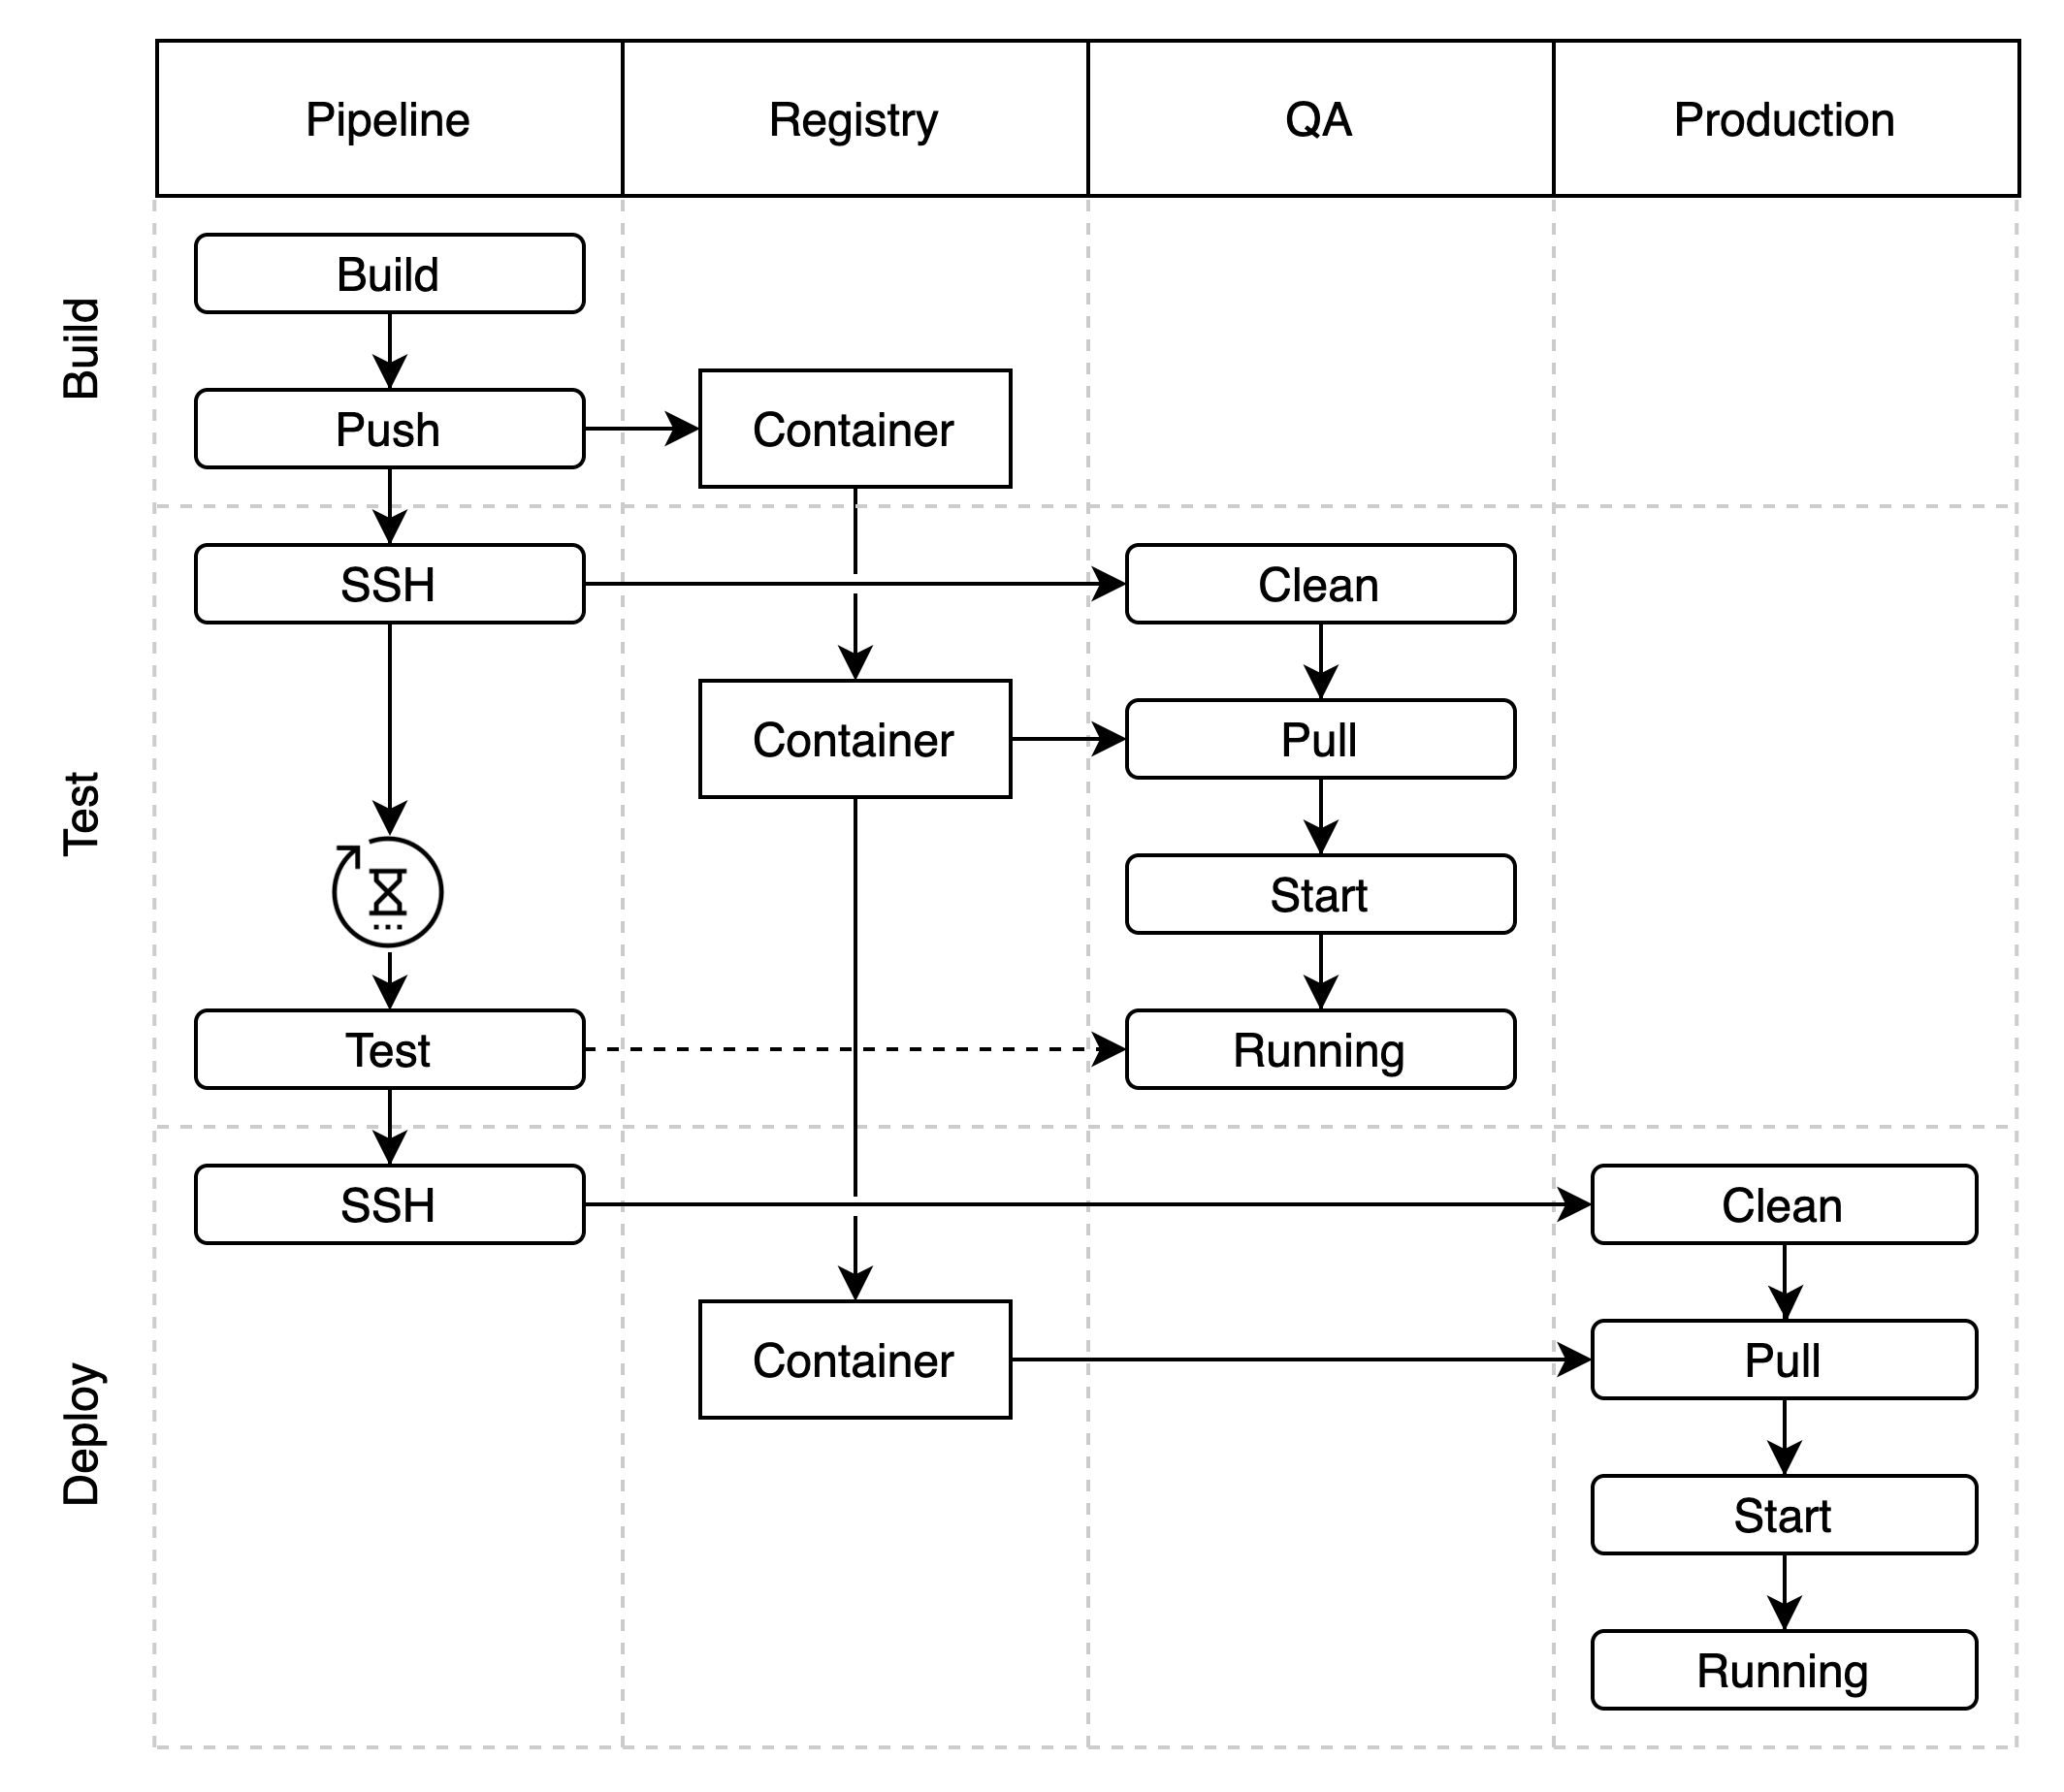
\includegraphics[scale=0.2]{img/abbildungen/Pipeline}
    \end{center}
    \caption{Übersicht über den stetigen Auslieferungsprozess}
    \label{figure:uebersichtueberdenstetigenauslieferungsprozess}
\end{figure}

Die erste Umgebung ist die Pipeline, ein in einem
Gitlab Runner ausgelagerter Prozess, der ein vordefiniertes Script durchläuft.
Damit der Gitlab Runner weiß, was er zu tun hat, werden in der \code{.gitlab-ci.yml}
Datei einzelne Abschnitte und deren Aufgaben mithilfe der vereinfachten
Auszeichnungssprache YAML definiert. Für jeden Abschnitt kann ein eigenes Docker-Image
gewählt werden. Mehr dazu findet man in \Cref{subsec:stages}. An zweiter Stelle
befindet sich die Docker Registry.\footnote{Eine Docker Registry ist eine Versionsverwaltung für Docker-Images.}
Sind die Images getestet, ist davon auszugehen, dass sich diese auch
in ausgeliefertem Zustand genauso verhalten werden, wie dies beim Testen
der Fall war. Die Qualitätssicherung ist an dritter Stelle\footnote{Auf English Quality Assurance, abgekürzt QA.}
Hier wird die Software nach ihrer Qualität getestet. Erst wenn sie alle
zuvor definierten Qualitätsmerkmale aufweist, darf die Software in die Produktionsumgebung
ausgeliefert werden. Die Produktionsumgebung unterscheidet sich von der QA-Umgebung
nur geringfügig. Im Gegensatz zur QA werden hier die Daten in den Datenbanken persistiert und die
einzelnen Container je nach benötigter Rechenleistung skaliert.

\subsection{Stages}
\label{subsec:stages}
Die drei in Abbildung \ref{figure:uebersichtueberdenstetigenauslieferungsprozess} dargestellten Stages sind
die \mbox{Build-,} die \mbox{Test-,} sowie die Deploy-Stage. Genauso wie das Produktivsystem
besteht auch die Pipeline aus unterschiedlichen Docker-Umgebungen. Die Test-Stage ist in eine Vorbereitungs-
und einer Durchführungsphase unterteilt. In der Vorbereitungsphase wird das für die Tests
benötigte Cluster erstellt. Die Durchführungsphase ist in zwei parallellaufende Prozesse
unterteilt. Dies ist nötig, da die Integrationstests für den Resource Management Service
eine Node.js-Umgebung und den Data Delivery Service eine Golang-Umgebung benötigen.

Die Arbeit lagert öfter auftretende Funktionalitäten der Gitlab-CI-Pipeline in eigene Scripts aus.
So wird redundanter Quellcode in der Pipeline verhindert. Ein Beispiel hierfür
ist Quellcode \ref{lst:wiederverwendbarescriptsdergitlabci}. Das erste ausgelagerte
Script ermöglicht die Verwendung von SSH innerhalb der Pipeline. Somit kann sich
die pipeline mit dem Server verbinden, um die Docker-Compose Datei auf den Server
zu kopieren und diese auszuführen. Das zweite Script ist dafür zuständig,
sich in die Docker Registry einzuloggen. Dies ist nötig, um Docker-Container
in die Registry zu speichern und diese später vom Server aus wieder abzufragen.

\begin{listing}
    \inputminted{yaml}{snippets/yml/reusable_scripts.yml}
    \caption{Wiederverwendbare Scripts der Gitlab-CI}
    \label{lst:wiederverwendbarescriptsdergitlabci}
\end{listing}

Für die Build- und Deploy-Stage wird ein von Docker vorgefertigtes Git-Image verwendet. Nach der Deploy-Stage
kommt noch eine Seed-Stage. Sie aktualisiert die im Redis-Cache gespeicherten Plugins. Die Plugins können
allerdings von außerhalb der Pipeline aktualisiert werden.

\subsection{Health-Checks}
\label{subsec:healthcheck}
Um die Verfügbarkeit der Services sicherzustellen, werden auf
Serviceebene Health-Check-Endpunkte bereitgestellt. Diese spiegeln den aktuellen
Gesundheitszustand des jeweiligen Dienstes wieder. Ein Health-Check-Endpunkt
ist speziell dann nützlich, wenn ein Dienst oder ein Verfahren von einem anderen
abhängig ist. So ist beispielsweise die Backendapi von der Datenbank
abhängig. Andererseits ist der Frontenddienst sowie die Integrationstests
in der Test-Stage von der Backendapi abhängig. In der Arbeit wurden für alle Services
rudimentäre Health-Checks implementiert, mithilfe derer die Produktionsserver ohne Ausfallzeit
aktualisiert werden können. Bei einem Update fährt Docker Swarm die auszutauschende
Instanz erst herunter, wenn eine neue betriebsbereit ist. Ob eine neue Instanz betriebsbereit ist,
wird durch den Health-Check bestimmt. Für den Health-Check des Nginx-Containers ruft die Arbeit beispielsweise
in einem Shell-Script den Befehl \code{service nginx status} auf. Ist das Resultat Positiv, wird
das Script mit \code{0} beendet, andernfalls mit \code{1}. Bei den eigenen Services werden \code{/health-check}
Routen bereitgestellt, die den Zustand des Services wiederspiegeln. Hier wird unter anderem geprüft, ob die Datenbanken
und der Cache mit dem Service verbunden sind.

\begin{listing}
    \inputminted{sh}{snippets/sh/healthcheck.sh}
    \caption{Warteschleife in Pipeline}
    \label{lst:healthcheck}
\end{listing}

In der Gitlab-CI wird mithilfe eines kleinen Shell-Scripts eine Warteschleife ausgeführt, die mithilfe von
\code{curl} den Health-Check-Endpunkt des jeweiligen Services abfragt. In Quellcode \ref{lst:healthcheck}
ist ein solches Script zu sehen. Die Arbeit stellt so sicher, dass bei der Durchführung der Tests die
benötigten Services funktionsbereit sind.

\section{Frontendanwendung}
\label{sec:frontendanwendung}
Die Frontendanwendung ist mit dem Frontendframework React geschrieben.
Zur Visualisierung der GUI-Komponenten wird wie bereits in \Cref{subsec:zentralisierungderindividualisierbarkeit}
erwähnt, das CSS-Framework Bootstrap verwendet. Die Arbeit hat sich bewusst gegen
eine React-Bootstrap-Bibliothek entschieden, um ein schnelleres Auswechseln von CSS-Frameworks
zu ermöglichen. Bei React-Bootstrap-Bibliothek werden für die Komponenten ganze Klassen importiert,
die man dann ersetzen müsste. CSS-Tags hingegen lassen sich schneller überschreiben oder austauschen.
Bis auf die Bibliotheken \code{jmespath.js} und \code{qrcode} wurde die komplette Funktionalität der Frontendanwendung
selbst implementiert. Die Zustandsverwaltung wurde mit der Context API von React realisiert.
Immer wieder vorkommende Funktionalitäten wurden in React-Hooks ausgelagert. Diese Hooks werden in einem
\code{common} Ordner zusammen mit oft benutzten React-Komponenten ausgelagert. Die Routen der Frontendanwendung
besitzten nur für die Seiten, die Ressourcen Anzeigen, den von REST bekannten Aufbau der URL-Pfade. Die Pfade
wurden möglichst benutzerfreundlich benannt. So ist der URL-Pfad der Loginseite beispielsweise \code{/login}.
Aus SEO-Gründen und der Benutzerfreundlichkeit wegen verändert sich der Titel sowie die Beschreibung je nach
Seite der Frontendanwendung. Der Begriff Single-Page-Webanwendung bezieht sich hier nur auf das initiale Laden
einer HTML-Seite. Die Frontendanwendung besitzt mehrere Seite, die alle über Suchmaschienen wie Google
gefunden werden können.

Die Frontendanwendung besitzt einen React-Hook für die Anordnung der bereits im Dashboard existierenden Diagramme, einen für
die Positionierung neuer Diagramme und einen für das Zeichnen der farbigen Bereiche, die beim Drag and Drop erscheinen.
Des Weiteren wurden externe Schnittstellen in Hooks verpackt, um so die Schnittstelle vor der Anwendung
zu Abstrahieren. Schnittstellen der Web Storage API wie \code{LocalStorage} und \code{SessionStorage}
wurden so erweitert, dass ganze JavaScript-Objekte gespeichert werden können. Außerdem wird der Zustand zwischen
der Anwendung und der Web Storage API synchronisiert. Verändert der Nutzer die Sprache in einem
Browser-Tab, wird diese auch in allen anderen Browser-Tabs geändert.

Die zwei bedeutsamsten Hooks sind \code{useApiEndpoint} und \code{useDeliveryEndpoint}. Sie ermöglichen
die Kommunikation zu den Mircoservices im Backend. Der \code{useApiEndpoint} Hook gibt die CRUD-Operationen,
welche für die Kommunikation mit einer REST-API nötig sind, zurück. Der \code{useDeliveryEndpoint} Hook
stellt eine \code{publish} sowie eine \code{subscribe} Funktion zur Verfügung. Die \code{useApiEndpoint} Hook
dient gleichzeitig als Middleware zwischen der Anwendung und dem Backend. So werden hier HTTP-Statuscodes
abgefangen, um so bestimmte Aktionen durchzuführen. Im Falle eines abgelaufenen Authentifizierungstokens,
wird so ein neues beantragt. Daraufhin wird die Fehlgeschlagene Anfrage erneut ausgeführt.

\begin{figure}
    \begin{center}
    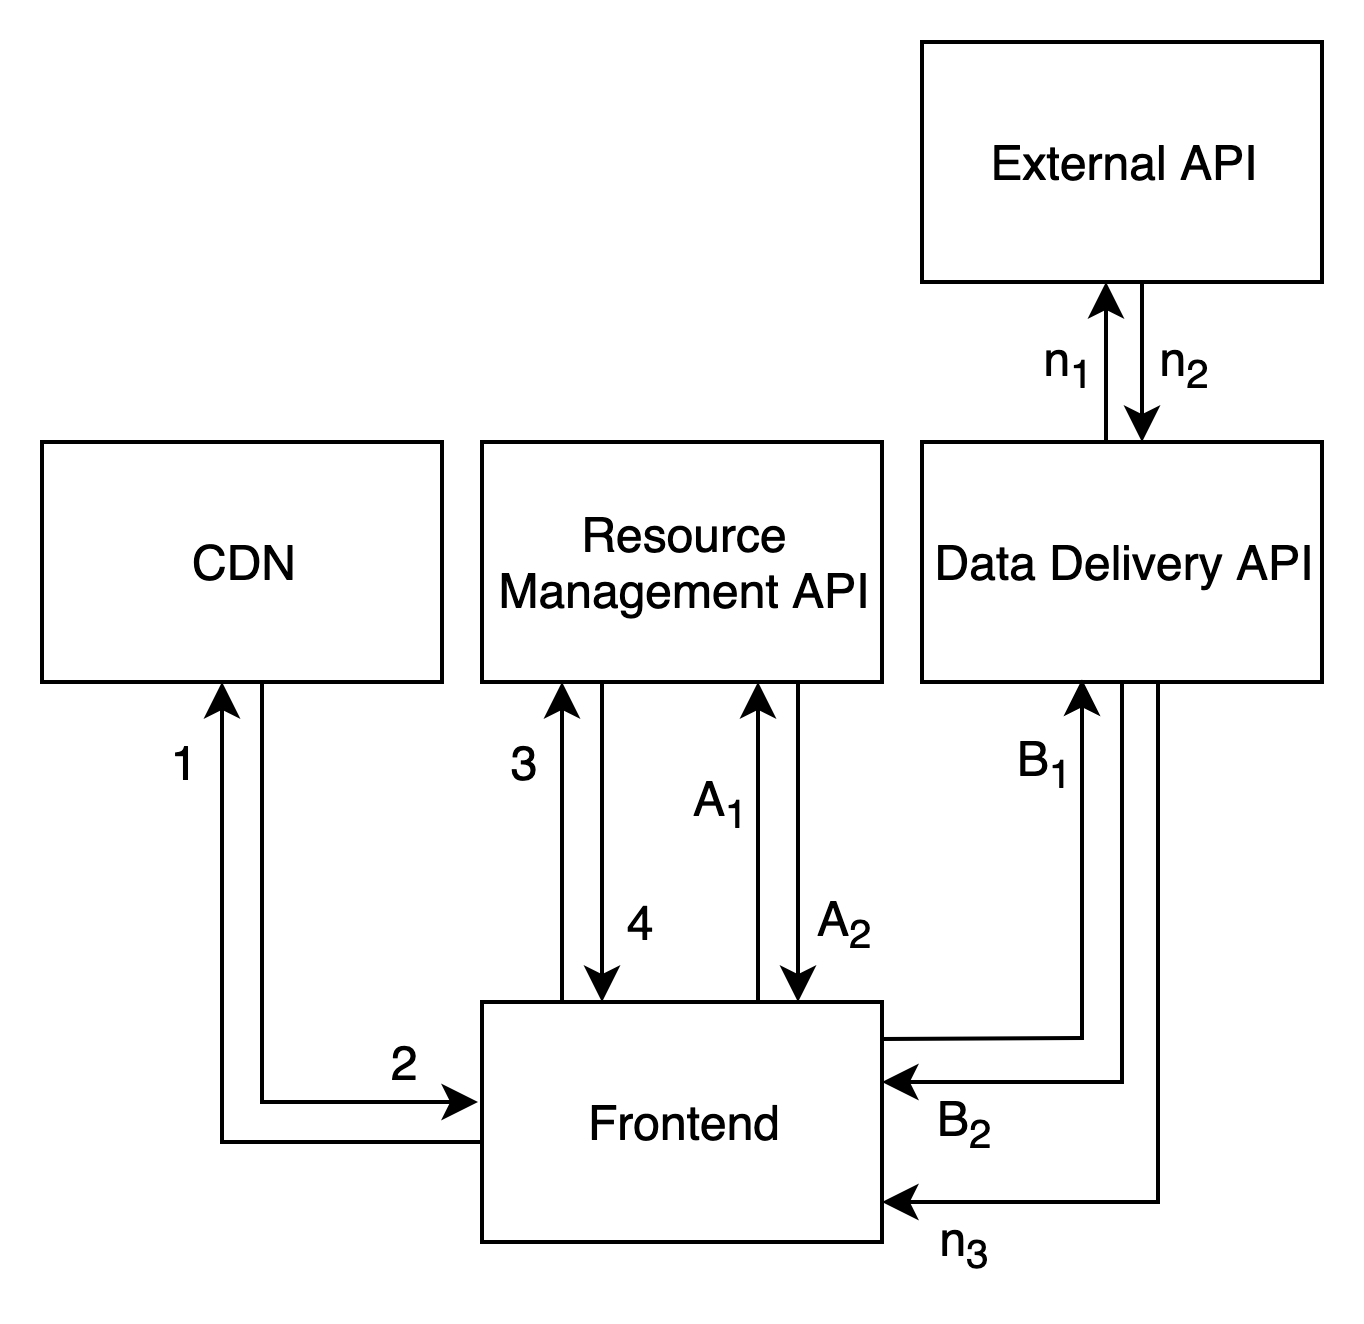
\includegraphics[scale=0.2]{img/abbildungen/InformationsaustauschDashboard}
    \end{center}
    \caption{Ablauf des Informationsaustausches eines Dashboards}
    \label{figure:informationsaustauschdashboard}
\end{figure}

Der \code{useDeliveryEndpoint} Hook implementiert ein eigenes Publish/Subscribe-Verfahren.
Um die Performance der Anwendung zu steigern, werden beim Ladevorgang eines Dashboards
die Diagramme sowie die anzuzeigenden Daten parallel geladen. In Abbildung \ref{figure:informationsaustauschdashboard}
ist der Informationsaustausch eines Dashboards dargestellt. Schritt eins und zwei steht
für das anfangliche Laden der Frontendanwendung über einen CDN. Dies tritt nur ein,
falls der Nutzer nicht bereits auf einer anderen Seite der Anwendung unterwegs war.
In Schritt drei wird die Dashboard-Ressource von dem Resource Management Service angefragt.
Die Dashboard-Ressource besteht neben den gewöhnlichen Feldern wie ID, Title, Beschreibung,
Erstellungsdatum und Eigentümer aus einem Feld mit dem Namen "Data". Dieses Feld beinhaltet
ein JSON, das den Aufbau und die Einstellungen eines Dashboards darstellt.\footnote{Ein
Beispiel hierfür ist der Quellcodeausschnitt \ref{lst:jsondateizurspeicherungeinesdashboards}
im Anhang unter "Weitere Quellcodeausschnitte".} Anhand dieser Informationen werden
daraufhin zeitgleich in \( A_1 \) die benötigten Plugins von dem Resource Management Service
und in \( B_1 \) die zu visualisierenden Daten von dem Data Delivery Service angefragt.\footnote{Das Anfragen der zu visualisierenden Daten erfolgt über die Publish-Funktion des 
\code{useDeliveryEndpoint} Hooks.}
Kommen die Plugins vor den zu visualisierenden Daten an, abbonieren diese über 
den \code{useDeliveryEndpoint} Hook mithilfe der Data Source Id die für das Plugin relevanten
Daten. Sobald diese ankommen, wird das durch das Plugin dargestellte Diagramm mit
den Daten versorgt. Kommen allerdings die zu visualisierenden Daten vor dem Plugin an,
speichert der \code{useDeliveryEndpoint} Hook die Daten und übergibt diese direkt beim
ersten Aufruf der durch den \code{useDeliveryEndpoint} Hook bereitgestellten
Subscribe-Funktion. \( n_3 \) steht für alle weiteren Schritte, die benötigt werden,
um die Daten des Diagramms aktuell zu halten. Je nach definiertem Interval sendet
der Data Delivery Service die Daten über die WebSocket-Verbindung zum Client.
In die Subscribe-Funktion wird neben der Data Source Id ein Callback übergeben,
der immer dann aufgerufen wird, wenn neue für das Plugin relevante Daten angekommen sind.
Diese werden dann mithilfe des Plugins auf dem Bildschirm aktualisiert.

\begin{listing}
    \inputminted{jsx}{snippets/jsx/useModalBeispiel.jsx}
    \caption{Verwendung des \code{useModal} Hooks}
    \label{lst:verwendungdesusemodalhooks}
\end{listing}

Zum Erstellen sowie als Sicherheitsabfrage vor der Löschung von Ressourcen verwendet die Arbeit Dialogfenster.
Hierfür stellt die Arbeit den \code{useModal} Hook bereit. Ein Beispiel befindet sich in
Quellcode \ref{lst:verwendungdesusemodalhooks}. Mithilfe des Hooks
kann mit nur weniger Zeilen ein Dialogfenster samt Funktionalität in eine React-Komponente integriert werden.
Der \code{useModal} Hook gibt in einem Array zwei Funktionen zurück; eine zum Öffnen und eine zum
Schließen des Modals. Als Eingabeparameter erwartet der Hook ein Callback und ein Array. Der Callback
gibt die anzuzeigende GUI-Komponente zurück. In das Array werden Referenzen übergeben, anhand derer
der Hook weiß, wann er die GUI-Komponente neu rendern muss.

Die Frontendanwendung besitzt neben den Hooks auch hilfreiche React-Komponenten. So gibt es
eine \code{ProtectedRoute}, welche den Benutzer umleistet, falls dieser keine Rechte für den
angefragten URL-Pfad besitzt.\footnote{Hierbei ist anzumerken, dass die eigentliche Rechteverwaltung durch
das Backend abgesichert ist.} Außerdem beinhaltet die Frontendanwendung Eingabevalidierung der Formulare
sowie Fehlermeldungen in Form von kleinen Informationsfenstern, die sich rechts oben im Bildschirm ansammeln
und nach fünf Sekunden verschwinden. Hat der angemeldete Nutzer Administrationsrechte, erscheint unter den
Benutzereinstellungen ein Menüpunkt, über den die Aministrationsoberfläche erreichbar ist. Alle in der
Frontendanwendung verwendeten Ressourcen können erstellt, angesehen, verändert und auch wieder gelöscht werden.
Für bestimmte Operationen wie das Löschen eines Benutzers, wird, auch wenn der Benutzer bereits eingeloggt ist,
ein zusätzliches Modal angezeigt, dass die Anmeldedaten abfragt. Um die initiale Zugriffssicherheit zu erhöhen,
bietet die Anwendung eine Zwei-Faktor-Authentisierung. In \Cref{subsec:authentifizierungsverfahren} geht die
Arbeit genauer auf das Authentifizierungsverfahren ein.

\subsection{Seitenumbruch und Suche}
\label{subsec:seitenumbruchundsuche}
Um die jeweiligen Ressourcen, wie Beispielsweise ein spezielles Dashboard, auszuwählen, kann man über
die Seitenleiste\footnote{Im installierten Modus werden die Ressourcen als Navigationsmenüs am unteren Bildschirmrand aufgelistet.}
auf eine Übersicht der Ressourcen gelangen. Da nicht alle Ressourcen auf eine Seite passen, werden diese mithilfe
einer Seitennavigation am unteren ende der Seite zugänglich gemacht. Je nachdem, wo sich der Benutzer befindet,
kann dieser so ganz an den Anfang, ganz an das Ende, eine Seite vor, eine Seite zurück navigieren sowie aus einer geringen Anzahl
an naheliegenden Seiten die passende auswählen. Die Anzahl der Seiten, zu denen eine direkte Navigation möglich ist, hängt von
der Bildschirmgröße des Endgerätes ab. Die maximale Anzahl ist hierbei vier Seiten in jede Richtung. Der Seitenumbruch befindet sich
bei zehn Ressourcen pro Seite. Bei einer größeren Anzahl an Ressourcen, kann das Navigieren durch
die Seiten sehr viel Zeit in Anspruch nehmen. Hierfür hat die Arbeit eine Suchfunktion implementiert. Die Suchfunktion befindet sich
in der oberen Navigationsleiste. Durch einen Zeichenvergleich des Titels der Ressource können so die passenden Ressourcen schneller gefunden
werden. Die Suche zeigt die zehn besten Resultate in einem Drop-Down-Menü an. Für den Zeichenvergleich verwendet der Resource Management Service
die von PostgreSQL angebotene Funktionalität zum Vergleichen von Zeichenketten. Ein Bildschirmschnappschuss der Suchfunktionalität befindet sich
im Anhang unter "Screenshots" in \Cref{figure:sucheundbearbeitungderdatenquelle}.

\subsection{Installation}
\label{subec:installation}
Die Anwendung ist von dem Browser sowie von dem Google Play Store aus installierbar. Als Einstieg
in die Frontendanwendung bietet das Web App Manifest sowie das Android Manifest eine URL als Einstiegspunkt.
Hier verwendet die Anwendung den Pfad \code{/installed}. Wird die progressive Webanwendung über diesen Pfad
aufgerufen, wird ein Feld im SessionStorage gesetzt. Mithilfe eines \code{useInstalled} Hooks, kann innerhalb
der Anwendung nachgefragt werden, ob die Anwendung vom Nutzer installiert wurde oder nicht. Anhand dieser
Information werden GUI-Komponenten angezeigt, die dem Nutzer ein natives Erscheinungsbild anbieten. So wird beispielsweise
eine Werkzeugleiste am unteren Ende des Bildschirms angezeigt, die es den mobilen Nutzern ermöglicht,
einfach mit dem Daumen zwischen den Seiten für die Dashboards, Diagrammen und Datenquellen zu wechseln.
Da sich die Seitenleiste, über die die Ressourcen im nicht-installierten Zustand erreichbar sind, bei mobilen
Endgeräten über den Inhalt schiebt, benötigt die Navigation zur Liste der Ressourcen zwei Klicks. Dies ist
bei der Desktop-Version nicht der Fall. Hier kann die Seitenleiste offen gelassen werden, wodurch nur ein Klick
benötigt wird. Durch die Werkzeugleiste ist es mobilen Nutzern ermöglicht, die Liste der Ressourcen mit nur einem
Klick zu erreichen.


\subsection{Zwischenspeicherstrategie im Service Worker}
\label{subsec:zwischenspeicherstrategieimserviceworker}
Ein Service Worker ist ein in JavaScript geschriebener,
eventbasierter Proxy, welcher in einem separaten Thread im Browser
läuft und an eine spezifische Origin gekoppelt ist. Er hat
die Möglichkeit Anfragen zwischen der im Browser ausgeführten
Anwendung und dem Server abzufangen und zu verarbeiten.

Cache Only
Network Only
Cache First
Network First
Cache then Network
Stale while Revalidate
Generic Fallback

\begin{description}
    \item[Für den Zwischenspeicher des Browsers relevante Untergliederung]~\par
    \begin{itemize}
       \item Statische Dateien mit Hash
       \begin{itemize}
            \item main.dd5a1ad0.chunk.css
            \item main.46e36a4b.chunk.js
            \item 2.dc039c03.chunk.js
       \end{itemize}
       \item Statische Dateien ohne Hash
       \begin{itemize}
            \item index.html
            \item manifest.json
            \item favicon.ico
       \end{itemize}
       \item JSON Ressourcen von AJAX Anfragen
    \end{itemize}
\end{description}

Daraus folgende Zwischenspeicherstrategien:

\begin{description}
    \item[Zwischenspeicherstrategie]~\par
    \begin{enumerate}
       \item Statische Dateien mit Hash
       \begin{enumerate}
          \item Zuerst aus dem Zwischenspeicher anfragen
          \item Falls nicht vorhanden, aus dem Netzwerk laden und in den Zwischenspeicher ablegen
       \end{enumerate}
       \item Statische Dateien ohne Hash
       \begin{enumerate}
            \item Zuerst aus dem Netzwerk anfragen und in den Zwischenspeicher ablegen
            \item Falls keine Netzwerkverbindung vorhanden, aus dem Zwischenspeicher laden
        \end{enumerate}
        \item JSON Ressourcen von AJAX Anfragen
        \begin{enumerate}
             \item Zuerst aus dem Netzwerk anfragen
             \item Falls nicht vorhanden, Offline-Rückfallseite anzeigen 
         \end{enumerate}
    \end{enumerate}
 \end{description}

\section{Plugins}
\label{sec:plugins}

\section{Resource Management Service}
\label{sec:resourcemanagementservice}

\subsection{Authentifizierungsverfahren}
\label{subsec:authentifizierungsverfahren}

\section{Data Delivery Service}
\label{sec:datadeliveryservice}

